
\subsection{Datasets}
We used Europarl dataset and the data was numberized after tokenizing, splitting, and excluding xml markups. The first $10K$ sentences were used as the test data, and the last 80\% as the training data (See Table~\ref{fig:data}).

\begin{table}
\resizebox{1\columnwidth}{!}{
\begin{tabular}{ll|cc|c}
Language&&Size (MB)&Tokens (M)& Sentences (K)\\
\toprule 
Bulgarian&BG&36.11&8.53&329\\
Czech&CS&53.48&12.25&535\\
German&DE&171.80&44.07&1785 \\
English&EN&179.15&49.32&1815\\
Finnish&FI&145.32&32.85&1737\\
French&FR&197.68&53.82&1792\\
Hungarian&HU&52.53&12.02&527\\
Italian&IT&186.67&48.08&1703\\
Portuguese&PT&187.20&49.03&1737\\
\end{tabular}}
\caption{Tokens and sentence counts refer to the training partition. \trevor{Move to \supp}}\label{fig:data}
\end{table}
Figure~\ref{fig:data} is showing XXX.
\begin{figure}
\includegraphics[width=\columnwidth]{figures/german_pattern_size.pdf}
\caption{Number of successful queries across different pattern sizes from KN computation over the German test set, with unbounded $m$.}
\end{figure}\label{fig:germanpattern}

\paragraph{Perplexity}
We evaluated the perplexity across different languages and using \ngrams of varying order from $m=2$ to $\infty$ (unbounded), as shown on Figure~\ref{figure:pplx}.
Our results matched the perplexity results from \SRILM (for smaller values of $m$ in which \SRILM training was feasible, $m \le 10$).
Note that perplexity drops dramatically from $m=2\ldots5$ however the gains thereafter are modest for most languages.
Despite this, several large \ngram matches were found as illustrated in Figure~\ref{fig:germanpattern}, ranging in size up to a 34-gram match.
We speculate that the perplexity plateau is due to the simplistic Kneser-Ney discounting formula which is not designed for higher order \ngram LMs and appear to discount large \ngrams too aggressively. 
We leave further exploration of richer discounting techniques such as Modified Kneser-Ney \cite{chen_goodman} or the Sequence Memoizer \cite{wood_teh} to our future work.

%\subsection{Perplexity Evaluation}
\begin{figure}
% Created by tikzDevice version 0.8.1 on 2015-05-29 13:08:13
% !TEX encoding = UTF-8 Unicode
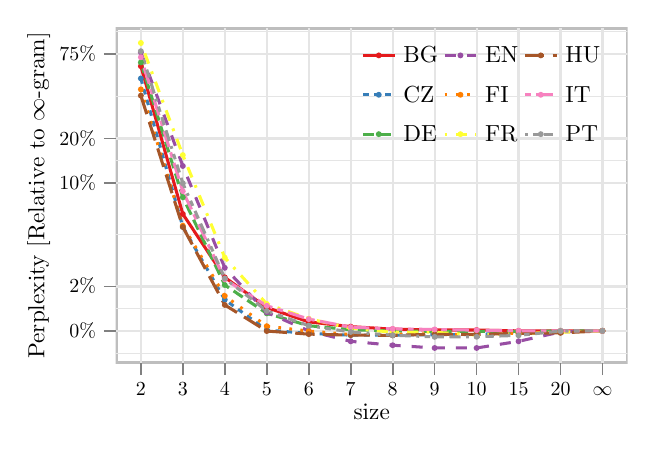
\begin{tikzpicture}[x=1pt,y=1pt]
\definecolor{fillColor}{RGB}{255,255,255}
\path[use as bounding box,fill=fillColor,fill opacity=0.00] (0,0) rectangle (216.81,144.54);
\begin{scope}
\path[clip] (  0.00,  0.00) rectangle (216.81,144.54);
\definecolor{fillColor}{RGB}{255,255,255}

\path[fill=fillColor] (  0.00,  0.00) rectangle (216.81,144.54);
\end{scope}
\begin{scope}
\path[clip] ( 31.80, 23.29) rectangle (216.81,144.54);
\definecolor{drawColor}{RGB}{190,190,190}

\path[draw=drawColor,line width= 1.5pt,line join=round,line cap=round] ( 31.80, 23.29) rectangle (216.81,144.54);
\definecolor{drawColor}{gray}{0.90}

\path[draw=drawColor,line width= 0.3pt,line join=round] ( 31.80, 26.94) --
	(216.81, 26.94);

\path[draw=drawColor,line width= 0.3pt,line join=round] ( 31.80, 43.01) --
	(216.81, 43.01);

\path[draw=drawColor,line width= 0.3pt,line join=round] ( 31.80, 69.72) --
	(216.81, 69.72);

\path[draw=drawColor,line width= 0.3pt,line join=round] ( 31.80, 96.43) --
	(216.81, 96.43);

\path[draw=drawColor,line width= 0.3pt,line join=round] ( 31.80,119.79) --
	(216.81,119.79);

\path[draw=drawColor,line width= 0.3pt,line join=round] ( 31.80,143.16) --
	(216.81,143.16);

\path[draw=drawColor,line width= 0.8pt,line join=round] ( 31.80, 34.98) --
	(216.81, 34.98);

\path[draw=drawColor,line width= 0.8pt,line join=round] ( 31.80, 51.05) --
	(216.81, 51.05);

\path[draw=drawColor,line width= 0.8pt,line join=round] ( 31.80, 88.39) --
	(216.81, 88.39);

\path[draw=drawColor,line width= 0.8pt,line join=round] ( 31.80,104.46) --
	(216.81,104.46);

\path[draw=drawColor,line width= 0.8pt,line join=round] ( 31.80,135.12) --
	(216.81,135.12);

\path[draw=drawColor,line width= 0.8pt,line join=round] ( 40.90, 23.29) --
	( 40.90,144.54);

\path[draw=drawColor,line width= 0.8pt,line join=round] ( 56.06, 23.29) --
	( 56.06,144.54);

\path[draw=drawColor,line width= 0.8pt,line join=round] ( 71.23, 23.29) --
	( 71.23,144.54);

\path[draw=drawColor,line width= 0.8pt,line join=round] ( 86.39, 23.29) --
	( 86.39,144.54);

\path[draw=drawColor,line width= 0.8pt,line join=round] (101.56, 23.29) --
	(101.56,144.54);

\path[draw=drawColor,line width= 0.8pt,line join=round] (116.72, 23.29) --
	(116.72,144.54);

\path[draw=drawColor,line width= 0.8pt,line join=round] (131.89, 23.29) --
	(131.89,144.54);

\path[draw=drawColor,line width= 0.8pt,line join=round] (147.05, 23.29) --
	(147.05,144.54);

\path[draw=drawColor,line width= 0.8pt,line join=round] (162.22, 23.29) --
	(162.22,144.54);

\path[draw=drawColor,line width= 0.8pt,line join=round] (177.38, 23.29) --
	(177.38,144.54);

\path[draw=drawColor,line width= 0.8pt,line join=round] (192.55, 23.29) --
	(192.55,144.54);

\path[draw=drawColor,line width= 0.8pt,line join=round] (207.71, 23.29) --
	(207.71,144.54);
\definecolor{drawColor}{RGB}{228,26,28}

\path[draw=drawColor,line width= 1.1pt,line join=round] ( 40.90,130.63) --
	( 56.06, 77.21) --
	( 71.23, 54.31) --
	( 86.39, 43.41) --
	(101.56, 38.23) --
	(116.72, 36.51) --
	(131.89, 35.60) --
	(147.05, 35.29) --
	(162.22, 35.29) --
	(177.38, 34.98) --
	(192.55, 34.98) --
	(207.71, 34.98);
\definecolor{drawColor}{RGB}{55,126,184}

\path[draw=drawColor,line width= 1.1pt,dash pattern=on 2pt off 2pt ,line join=round] ( 40.90,126.19) --
	( 56.06, 72.56) --
	( 71.23, 46.26) --
	( 86.39, 35.27) --
	(101.56, 34.06) --
	(116.72, 33.43) --
	(131.89, 33.43) --
	(147.05, 33.59) --
	(162.22, 33.59) --
	(177.38, 34.67) --
	(192.55, 34.82) --
	(207.71, 34.98);
\definecolor{drawColor}{RGB}{77,175,74}

\path[draw=drawColor,line width= 1.1pt,dash pattern=on 4pt off 2pt ,line join=round] ( 40.90,131.98) --
	( 56.06, 83.27) --
	( 71.23, 51.55) --
	( 86.39, 41.31) --
	(101.56, 36.83) --
	(116.72, 35.40) --
	(131.89, 34.98) --
	(147.05, 34.76) --
	(162.22, 34.76) --
	(177.38, 34.76) --
	(192.55, 34.98) --
	(207.71, 34.98);
\definecolor{drawColor}{RGB}{152,78,163}

\path[draw=drawColor,line width= 1.1pt,dash pattern=on 4pt off 4pt ,line join=round] ( 40.90,135.63) --
	( 56.06, 94.56) --
	( 71.23, 57.75) --
	( 86.39, 41.66) --
	(101.56, 34.98) --
	(116.72, 31.20) --
	(131.89, 29.79) --
	(147.05, 28.80) --
	(162.22, 28.80) --
	(177.38, 31.20) --
	(192.55, 34.58) --
	(207.71, 34.98);
\definecolor{drawColor}{RGB}{255,127,0}

\path[draw=drawColor,line width= 1.1pt,dash pattern=on 1pt off 3pt ,line join=round] ( 40.90,122.24) --
	( 56.06, 72.99) --
	( 71.23, 47.59) --
	( 86.39, 36.68) --
	(101.56, 34.90) --
	(116.72, 33.68) --
	(131.89, 33.76) --
	(147.05, 33.92) --
	(162.22, 33.53) --
	(177.38, 34.22) --
	(192.55, 34.75) --
	(207.71, 34.98);
\definecolor{drawColor}{RGB}{255,255,51}

\path[draw=drawColor,line width= 1.1pt,dash pattern=on 1pt off 3pt on 4pt off 3pt ,line join=round] ( 40.90,139.03) --
	( 56.06, 98.50) --
	( 71.23, 61.44) --
	( 86.39, 44.72) --
	(101.56, 39.37) --
	(116.72, 35.92) --
	(131.89, 34.49) --
	(147.05, 34.49) --
	(162.22, 33.48) --
	(177.38, 33.99) --
	(192.55, 34.49) --
	(207.71, 34.98);
\definecolor{drawColor}{RGB}{166,86,40}

\path[draw=drawColor,line width= 1.1pt,dash pattern=on 7pt off 3pt ,line join=round] ( 40.90,119.98) --
	( 56.06, 72.52) --
	( 71.23, 44.35) --
	( 86.39, 34.91) --
	(101.56, 33.80) --
	(116.72, 33.47) --
	(131.89, 33.36) --
	(147.05, 33.74) --
	(162.22, 33.69) --
	(177.38, 34.07) --
	(192.55, 34.25) --
	(207.71, 34.98);
\definecolor{drawColor}{RGB}{247,129,191}

\path[draw=drawColor,line width= 1.1pt,dash pattern=on 2pt off 2pt on 6pt off 2pt ,line join=round] ( 40.90,133.85) --
	( 56.06, 85.45) --
	( 71.23, 53.61) --
	( 86.39, 44.06) --
	(101.56, 39.24) --
	(116.72, 36.33) --
	(131.89, 35.69) --
	(147.05, 35.50) --
	(162.22, 35.23) --
	(177.38, 35.00) --
	(192.55, 34.96) --
	(207.71, 34.98);
\definecolor{drawColor}{gray}{0.60}

\path[draw=drawColor,line width= 1.1pt,dash pattern=on 1pt off 2pt on 2pt off 2pt on 3pt off 2pt on 4pt off 2pt ,line join=round] ( 40.90,136.04) --
	( 56.06, 88.32) --
	( 71.23, 53.95) --
	( 86.39, 42.18) --
	(101.56, 36.86) --
	(116.72, 34.57) --
	(131.89, 33.40) --
	(147.05, 32.81) --
	(162.22, 32.85) --
	(177.38, 33.35) --
	(192.55, 34.90) --
	(207.71, 34.98);
\definecolor{fillColor}{RGB}{228,26,28}

\path[fill=fillColor] ( 40.90,130.63) circle (  1.07);

\path[fill=fillColor] ( 56.06, 77.21) circle (  1.07);

\path[fill=fillColor] ( 71.23, 54.31) circle (  1.07);

\path[fill=fillColor] ( 86.39, 43.41) circle (  1.07);

\path[fill=fillColor] (101.56, 38.23) circle (  1.07);

\path[fill=fillColor] (116.72, 36.51) circle (  1.07);

\path[fill=fillColor] (131.89, 35.60) circle (  1.07);

\path[fill=fillColor] (147.05, 35.29) circle (  1.07);

\path[fill=fillColor] (162.22, 35.29) circle (  1.07);

\path[fill=fillColor] (177.38, 34.98) circle (  1.07);

\path[fill=fillColor] (192.55, 34.98) circle (  1.07);

\path[fill=fillColor] (207.71, 34.98) circle (  1.07);
\definecolor{fillColor}{RGB}{55,126,184}

\path[fill=fillColor] ( 40.90,126.19) circle (  1.07);

\path[fill=fillColor] ( 56.06, 72.56) circle (  1.07);

\path[fill=fillColor] ( 71.23, 46.26) circle (  1.07);

\path[fill=fillColor] ( 86.39, 35.27) circle (  1.07);

\path[fill=fillColor] (101.56, 34.06) circle (  1.07);

\path[fill=fillColor] (116.72, 33.43) circle (  1.07);

\path[fill=fillColor] (131.89, 33.43) circle (  1.07);

\path[fill=fillColor] (147.05, 33.59) circle (  1.07);

\path[fill=fillColor] (162.22, 33.59) circle (  1.07);

\path[fill=fillColor] (177.38, 34.67) circle (  1.07);

\path[fill=fillColor] (192.55, 34.82) circle (  1.07);

\path[fill=fillColor] (207.71, 34.98) circle (  1.07);
\definecolor{fillColor}{RGB}{77,175,74}

\path[fill=fillColor] ( 40.90,131.98) circle (  1.07);

\path[fill=fillColor] ( 56.06, 83.27) circle (  1.07);

\path[fill=fillColor] ( 71.23, 51.55) circle (  1.07);

\path[fill=fillColor] ( 86.39, 41.31) circle (  1.07);

\path[fill=fillColor] (101.56, 36.83) circle (  1.07);

\path[fill=fillColor] (116.72, 35.40) circle (  1.07);

\path[fill=fillColor] (131.89, 34.98) circle (  1.07);

\path[fill=fillColor] (147.05, 34.76) circle (  1.07);

\path[fill=fillColor] (162.22, 34.76) circle (  1.07);

\path[fill=fillColor] (177.38, 34.76) circle (  1.07);

\path[fill=fillColor] (192.55, 34.98) circle (  1.07);

\path[fill=fillColor] (207.71, 34.98) circle (  1.07);
\definecolor{fillColor}{RGB}{152,78,163}

\path[fill=fillColor] ( 40.90,135.63) circle (  1.07);

\path[fill=fillColor] ( 56.06, 94.56) circle (  1.07);

\path[fill=fillColor] ( 71.23, 57.75) circle (  1.07);

\path[fill=fillColor] ( 86.39, 41.66) circle (  1.07);

\path[fill=fillColor] (101.56, 34.98) circle (  1.07);

\path[fill=fillColor] (116.72, 31.20) circle (  1.07);

\path[fill=fillColor] (131.89, 29.79) circle (  1.07);

\path[fill=fillColor] (147.05, 28.80) circle (  1.07);

\path[fill=fillColor] (162.22, 28.80) circle (  1.07);

\path[fill=fillColor] (177.38, 31.20) circle (  1.07);

\path[fill=fillColor] (192.55, 34.58) circle (  1.07);

\path[fill=fillColor] (207.71, 34.98) circle (  1.07);
\definecolor{fillColor}{RGB}{255,127,0}

\path[fill=fillColor] ( 40.90,122.24) circle (  1.07);

\path[fill=fillColor] ( 56.06, 72.99) circle (  1.07);

\path[fill=fillColor] ( 71.23, 47.59) circle (  1.07);

\path[fill=fillColor] ( 86.39, 36.68) circle (  1.07);

\path[fill=fillColor] (101.56, 34.90) circle (  1.07);

\path[fill=fillColor] (116.72, 33.68) circle (  1.07);

\path[fill=fillColor] (131.89, 33.76) circle (  1.07);

\path[fill=fillColor] (147.05, 33.92) circle (  1.07);

\path[fill=fillColor] (162.22, 33.53) circle (  1.07);

\path[fill=fillColor] (177.38, 34.22) circle (  1.07);

\path[fill=fillColor] (192.55, 34.75) circle (  1.07);

\path[fill=fillColor] (207.71, 34.98) circle (  1.07);
\definecolor{fillColor}{RGB}{255,255,51}

\path[fill=fillColor] ( 40.90,139.03) circle (  1.07);

\path[fill=fillColor] ( 56.06, 98.50) circle (  1.07);

\path[fill=fillColor] ( 71.23, 61.44) circle (  1.07);

\path[fill=fillColor] ( 86.39, 44.72) circle (  1.07);

\path[fill=fillColor] (101.56, 39.37) circle (  1.07);

\path[fill=fillColor] (116.72, 35.92) circle (  1.07);

\path[fill=fillColor] (131.89, 34.49) circle (  1.07);

\path[fill=fillColor] (147.05, 34.49) circle (  1.07);

\path[fill=fillColor] (162.22, 33.48) circle (  1.07);

\path[fill=fillColor] (177.38, 33.99) circle (  1.07);

\path[fill=fillColor] (192.55, 34.49) circle (  1.07);

\path[fill=fillColor] (207.71, 34.98) circle (  1.07);
\definecolor{fillColor}{RGB}{166,86,40}

\path[fill=fillColor] ( 40.90,119.98) circle (  1.07);

\path[fill=fillColor] ( 56.06, 72.52) circle (  1.07);

\path[fill=fillColor] ( 71.23, 44.35) circle (  1.07);

\path[fill=fillColor] ( 86.39, 34.91) circle (  1.07);

\path[fill=fillColor] (101.56, 33.80) circle (  1.07);

\path[fill=fillColor] (116.72, 33.47) circle (  1.07);

\path[fill=fillColor] (131.89, 33.36) circle (  1.07);

\path[fill=fillColor] (147.05, 33.74) circle (  1.07);

\path[fill=fillColor] (162.22, 33.69) circle (  1.07);

\path[fill=fillColor] (177.38, 34.07) circle (  1.07);

\path[fill=fillColor] (192.55, 34.25) circle (  1.07);

\path[fill=fillColor] (207.71, 34.98) circle (  1.07);
\definecolor{fillColor}{RGB}{247,129,191}

\path[fill=fillColor] ( 40.90,133.85) circle (  1.07);

\path[fill=fillColor] ( 56.06, 85.45) circle (  1.07);

\path[fill=fillColor] ( 71.23, 53.61) circle (  1.07);

\path[fill=fillColor] ( 86.39, 44.06) circle (  1.07);

\path[fill=fillColor] (101.56, 39.24) circle (  1.07);

\path[fill=fillColor] (116.72, 36.33) circle (  1.07);

\path[fill=fillColor] (131.89, 35.69) circle (  1.07);

\path[fill=fillColor] (147.05, 35.50) circle (  1.07);

\path[fill=fillColor] (162.22, 35.23) circle (  1.07);

\path[fill=fillColor] (177.38, 35.00) circle (  1.07);

\path[fill=fillColor] (192.55, 34.96) circle (  1.07);

\path[fill=fillColor] (207.71, 34.98) circle (  1.07);
\definecolor{fillColor}{gray}{0.60}

\path[fill=fillColor] ( 40.90,136.04) circle (  1.07);

\path[fill=fillColor] ( 56.06, 88.32) circle (  1.07);

\path[fill=fillColor] ( 71.23, 53.95) circle (  1.07);

\path[fill=fillColor] ( 86.39, 42.18) circle (  1.07);

\path[fill=fillColor] (101.56, 36.86) circle (  1.07);

\path[fill=fillColor] (116.72, 34.57) circle (  1.07);

\path[fill=fillColor] (131.89, 33.40) circle (  1.07);

\path[fill=fillColor] (147.05, 32.81) circle (  1.07);

\path[fill=fillColor] (162.22, 32.85) circle (  1.07);

\path[fill=fillColor] (177.38, 33.35) circle (  1.07);

\path[fill=fillColor] (192.55, 34.90) circle (  1.07);

\path[fill=fillColor] (207.71, 34.98) circle (  1.07);
\end{scope}
\begin{scope}
\path[clip] (  0.00,  0.00) rectangle (216.81,144.54);
\definecolor{drawColor}{RGB}{0,0,0}

\node[text=drawColor,anchor=base east,inner sep=0pt, outer sep=0pt, scale=  0.72] at ( 24.69, 32.63) {0\%};

\node[text=drawColor,anchor=base east,inner sep=0pt, outer sep=0pt, scale=  0.72] at ( 24.69, 48.71) {2\%};

\node[text=drawColor,anchor=base east,inner sep=0pt, outer sep=0pt, scale=  0.72] at ( 24.69, 86.04) {10\%};

\node[text=drawColor,anchor=base east,inner sep=0pt, outer sep=0pt, scale=  0.72] at ( 24.69,102.12) {20\%};

\node[text=drawColor,anchor=base east,inner sep=0pt, outer sep=0pt, scale=  0.72] at ( 24.69,132.78) {75\%};
\end{scope}
\begin{scope}
\path[clip] (  0.00,  0.00) rectangle (216.81,144.54);
\definecolor{drawColor}{gray}{0.50}

\path[draw=drawColor,line width= 0.6pt,line join=round] ( 27.53, 34.98) --
	( 31.80, 34.98);

\path[draw=drawColor,line width= 0.6pt,line join=round] ( 27.53, 51.05) --
	( 31.80, 51.05);

\path[draw=drawColor,line width= 0.6pt,line join=round] ( 27.53, 88.39) --
	( 31.80, 88.39);

\path[draw=drawColor,line width= 0.6pt,line join=round] ( 27.53,104.46) --
	( 31.80,104.46);

\path[draw=drawColor,line width= 0.6pt,line join=round] ( 27.53,135.12) --
	( 31.80,135.12);
\end{scope}
\begin{scope}
\path[clip] (  0.00,  0.00) rectangle (216.81,144.54);
\definecolor{drawColor}{gray}{0.50}

\path[draw=drawColor,line width= 0.6pt,line join=round] ( 40.90, 19.02) --
	( 40.90, 23.29);

\path[draw=drawColor,line width= 0.6pt,line join=round] ( 56.06, 19.02) --
	( 56.06, 23.29);

\path[draw=drawColor,line width= 0.6pt,line join=round] ( 71.23, 19.02) --
	( 71.23, 23.29);

\path[draw=drawColor,line width= 0.6pt,line join=round] ( 86.39, 19.02) --
	( 86.39, 23.29);

\path[draw=drawColor,line width= 0.6pt,line join=round] (101.56, 19.02) --
	(101.56, 23.29);

\path[draw=drawColor,line width= 0.6pt,line join=round] (116.72, 19.02) --
	(116.72, 23.29);

\path[draw=drawColor,line width= 0.6pt,line join=round] (131.89, 19.02) --
	(131.89, 23.29);

\path[draw=drawColor,line width= 0.6pt,line join=round] (147.05, 19.02) --
	(147.05, 23.29);

\path[draw=drawColor,line width= 0.6pt,line join=round] (162.22, 19.02) --
	(162.22, 23.29);

\path[draw=drawColor,line width= 0.6pt,line join=round] (177.38, 19.02) --
	(177.38, 23.29);

\path[draw=drawColor,line width= 0.6pt,line join=round] (192.55, 19.02) --
	(192.55, 23.29);

\path[draw=drawColor,line width= 0.6pt,line join=round] (207.71, 19.02) --
	(207.71, 23.29);
\end{scope}
\begin{scope}
\path[clip] (  0.00,  0.00) rectangle (216.81,144.54);
\definecolor{drawColor}{RGB}{0,0,0}

\node[text=drawColor,anchor=base,inner sep=0pt, outer sep=0pt, scale=  0.72] at ( 40.90, 11.49) {2};

\node[text=drawColor,anchor=base,inner sep=0pt, outer sep=0pt, scale=  0.72] at ( 56.06, 11.49) {3};

\node[text=drawColor,anchor=base,inner sep=0pt, outer sep=0pt, scale=  0.72] at ( 71.23, 11.49) {4};

\node[text=drawColor,anchor=base,inner sep=0pt, outer sep=0pt, scale=  0.72] at ( 86.39, 11.49) {5};

\node[text=drawColor,anchor=base,inner sep=0pt, outer sep=0pt, scale=  0.72] at (101.56, 11.49) {6};

\node[text=drawColor,anchor=base,inner sep=0pt, outer sep=0pt, scale=  0.72] at (116.72, 11.49) {7};

\node[text=drawColor,anchor=base,inner sep=0pt, outer sep=0pt, scale=  0.72] at (131.89, 11.49) {8};

\node[text=drawColor,anchor=base,inner sep=0pt, outer sep=0pt, scale=  0.72] at (147.05, 11.49) {9};

\node[text=drawColor,anchor=base,inner sep=0pt, outer sep=0pt, scale=  0.72] at (162.22, 11.49) {10};

\node[text=drawColor,anchor=base,inner sep=0pt, outer sep=0pt, scale=  0.72] at (177.38, 11.49) {15};

\node[text=drawColor,anchor=base,inner sep=0pt, outer sep=0pt, scale=  0.72] at (192.55, 11.49) {20};

\node[text=drawColor,anchor=base,inner sep=0pt, outer sep=0pt, scale=  0.72] at (207.71, 11.49) {$\infty$};
\end{scope}
\begin{scope}
\path[clip] (  0.00,  0.00) rectangle (216.81,144.54);
\definecolor{drawColor}{RGB}{0,0,0}

\node[text=drawColor,anchor=base,inner sep=0pt, outer sep=0pt, scale=  0.84] at (124.31,  3.01) {\ngram size};
\end{scope}
\begin{scope}
\path[clip] (  0.00,  0.00) rectangle (216.81,144.54);
\definecolor{drawColor}{RGB}{0,0,0}

\node[text=drawColor,rotate= 90.00,anchor=base,inner sep=0pt, outer sep=0pt, scale=  0.84] at (  6.07, 83.92) {Perplexity [Relative to $\infty$-gram]};
\end{scope}
\begin{scope}
\path[clip] (  0.00,  0.00) rectangle (216.81,144.54);
\definecolor{drawColor}{RGB}{228,26,28}

\path[draw=drawColor,line width= 1.1pt,line join=round] (121.18,134.52) -- (132.56,134.52);
\end{scope}
\begin{scope}
\path[clip] (  0.00,  0.00) rectangle (216.81,144.54);
\definecolor{fillColor}{RGB}{228,26,28}

\path[fill=fillColor] (126.87,134.52) circle (  1.07);
\end{scope}
\begin{scope}
\path[clip] (  0.00,  0.00) rectangle (216.81,144.54);
\definecolor{drawColor}{RGB}{55,126,184}

\path[draw=drawColor,line width= 1.1pt,dash pattern=on 2pt off 2pt ,line join=round] (121.18,120.29) -- (132.56,120.29);
\end{scope}
\begin{scope}
\path[clip] (  0.00,  0.00) rectangle (216.81,144.54);
\definecolor{fillColor}{RGB}{55,126,184}

\path[fill=fillColor] (126.87,120.29) circle (  1.07);
\end{scope}
\begin{scope}
\path[clip] (  0.00,  0.00) rectangle (216.81,144.54);
\definecolor{drawColor}{RGB}{77,175,74}

\path[draw=drawColor,line width= 1.1pt,dash pattern=on 4pt off 2pt ,line join=round] (121.18,106.06) -- (132.56,106.06);
\end{scope}
\begin{scope}
\path[clip] (  0.00,  0.00) rectangle (216.81,144.54);
\definecolor{fillColor}{RGB}{77,175,74}

\path[fill=fillColor] (126.87,106.06) circle (  1.07);
\end{scope}
\begin{scope}
\path[clip] (  0.00,  0.00) rectangle (216.81,144.54);
\definecolor{drawColor}{RGB}{152,78,163}

\path[draw=drawColor,line width= 1.1pt,dash pattern=on 4pt off 4pt ,line join=round] (150.69,134.52) -- (162.07,134.52);
\end{scope}
\begin{scope}
\path[clip] (  0.00,  0.00) rectangle (216.81,144.54);
\definecolor{fillColor}{RGB}{152,78,163}

\path[fill=fillColor] (156.38,134.52) circle (  1.07);
\end{scope}
\begin{scope}
\path[clip] (  0.00,  0.00) rectangle (216.81,144.54);
\definecolor{drawColor}{RGB}{255,127,0}

\path[draw=drawColor,line width= 1.1pt,dash pattern=on 1pt off 3pt ,line join=round] (150.69,120.29) -- (162.07,120.29);
\end{scope}
\begin{scope}
\path[clip] (  0.00,  0.00) rectangle (216.81,144.54);
\definecolor{fillColor}{RGB}{255,127,0}

\path[fill=fillColor] (156.38,120.29) circle (  1.07);
\end{scope}
\begin{scope}
\path[clip] (  0.00,  0.00) rectangle (216.81,144.54);
\definecolor{drawColor}{RGB}{255,255,51}

\path[draw=drawColor,line width= 1.1pt,dash pattern=on 1pt off 3pt on 4pt off 3pt ,line join=round] (150.69,106.06) -- (162.07,106.06);
\end{scope}
\begin{scope}
\path[clip] (  0.00,  0.00) rectangle (216.81,144.54);
\definecolor{fillColor}{RGB}{255,255,51}

\path[fill=fillColor] (156.38,106.06) circle (  1.07);
\end{scope}
\begin{scope}
\path[clip] (  0.00,  0.00) rectangle (216.81,144.54);
\definecolor{drawColor}{RGB}{166,86,40}

\path[draw=drawColor,line width= 1.1pt,dash pattern=on 7pt off 3pt ,line join=round] (179.73,134.52) -- (191.11,134.52);
\end{scope}
\begin{scope}
\path[clip] (  0.00,  0.00) rectangle (216.81,144.54);
\definecolor{fillColor}{RGB}{166,86,40}

\path[fill=fillColor] (185.42,134.52) circle (  1.07);
\end{scope}
\begin{scope}
\path[clip] (  0.00,  0.00) rectangle (216.81,144.54);
\definecolor{drawColor}{RGB}{247,129,191}

\path[draw=drawColor,line width= 1.1pt,dash pattern=on 2pt off 2pt on 6pt off 2pt ,line join=round] (179.73,120.29) -- (191.11,120.29);
\end{scope}
\begin{scope}
\path[clip] (  0.00,  0.00) rectangle (216.81,144.54);
\definecolor{fillColor}{RGB}{247,129,191}

\path[fill=fillColor] (185.42,120.29) circle (  1.07);
\end{scope}
\begin{scope}
\path[clip] (  0.00,  0.00) rectangle (216.81,144.54);
\definecolor{drawColor}{gray}{0.60}

\path[draw=drawColor,line width= 1.1pt,dash pattern=on 1pt off 2pt on 2pt off 2pt on 3pt off 2pt on 4pt off 2pt ,line join=round] (179.73,106.06) -- (191.11,106.06);
\end{scope}
\begin{scope}
\path[clip] (  0.00,  0.00) rectangle (216.81,144.54);
\definecolor{fillColor}{gray}{0.60}

\path[fill=fillColor] (185.42,106.06) circle (  1.07);
\end{scope}
\begin{scope}
\path[clip] (  0.00,  0.00) rectangle (216.81,144.54);
\definecolor{drawColor}{RGB}{0,0,0}

\node[text=drawColor,anchor=base west,inner sep=0pt, outer sep=0pt, scale=  0.84] at (135.79,131.78) {BG};
\end{scope}
\begin{scope}
\path[clip] (  0.00,  0.00) rectangle (216.81,144.54);
\definecolor{drawColor}{RGB}{0,0,0}

\node[text=drawColor,anchor=base west,inner sep=0pt, outer sep=0pt, scale=  0.84] at (135.79,117.56) {CZ};
\end{scope}
\begin{scope}
\path[clip] (  0.00,  0.00) rectangle (216.81,144.54);
\definecolor{drawColor}{RGB}{0,0,0}

\node[text=drawColor,anchor=base west,inner sep=0pt, outer sep=0pt, scale=  0.84] at (135.79,103.33) {DE};
\end{scope}
\begin{scope}
\path[clip] (  0.00,  0.00) rectangle (216.81,144.54);
\definecolor{drawColor}{RGB}{0,0,0}

\node[text=drawColor,anchor=base west,inner sep=0pt, outer sep=0pt, scale=  0.84] at (165.30,131.78) {EN};
\end{scope}
\begin{scope}
\path[clip] (  0.00,  0.00) rectangle (216.81,144.54);
\definecolor{drawColor}{RGB}{0,0,0}

\node[text=drawColor,anchor=base west,inner sep=0pt, outer sep=0pt, scale=  0.84] at (165.30,117.56) {FI};
\end{scope}
\begin{scope}
\path[clip] (  0.00,  0.00) rectangle (216.81,144.54);
\definecolor{drawColor}{RGB}{0,0,0}

\node[text=drawColor,anchor=base west,inner sep=0pt, outer sep=0pt, scale=  0.84] at (165.30,103.33) {FR};
\end{scope}
\begin{scope}
\path[clip] (  0.00,  0.00) rectangle (216.81,144.54);
\definecolor{drawColor}{RGB}{0,0,0}

\node[text=drawColor,anchor=base west,inner sep=0pt, outer sep=0pt, scale=  0.84] at (194.34,131.78) {HU};
\end{scope}
\begin{scope}
\path[clip] (  0.00,  0.00) rectangle (216.81,144.54);
\definecolor{drawColor}{RGB}{0,0,0}

\node[text=drawColor,anchor=base west,inner sep=0pt, outer sep=0pt, scale=  0.84] at (194.34,117.56) {IT};
\end{scope}
\begin{scope}
\path[clip] (  0.00,  0.00) rectangle (216.81,144.54);
\definecolor{drawColor}{RGB}{0,0,0}

\node[text=drawColor,anchor=base west,inner sep=0pt, outer sep=0pt, scale=  0.84] at (194.34,103.33) {PT};
\end{scope}
\end{tikzpicture}

\caption{Perplexity results on several Europarl languages for different \ngram sizes, $m=2\ldots10,15,20,\infty$.}
\label{figure:pplx}
\end{figure}

\begin{figure}
\includegraphics[width=\columnwidth]{figures/german_pattern_size.pdf}
\caption{Number of successful queries across different pattern sizes from KN computation over the German test set, with unbounded $m$.}
\label{fig:germanpattern}
\end{figure}

\paragraph{Runtime Requirements}
Figure~\ref{figure:space-time} shows the time and memory usage during training and querying with \SRILM default (optimized for time), and compact (optimized for space). 

\begin{figure}
\includegraphics[width=\columnwidth]{figures/Time-Space.pdf}
\caption{Time versus space tradeoffs measured on Europarl German (de) dataset, showing memory and time requirements for the four methods: CST single, CST dual, \SRILM, and \SRILM compact. Times were measured using a 10k sentence test set.}
\label{figure:space-time}
\end{figure}




%%% Local Variables: 
%%% mode: latex
%%% TeX-master: "cstlm"
%%% End: 

